\documentclass[a4paper]{article}

\usepackage[english]{babel}
\usepackage[utf8]{inputenc}
\usepackage{amsmath}
\usepackage{graphicx}
\usepackage{enumitem}
\usepackage[colorinlistoftodos]{todonotes}
\usepackage{tikz}
\newcommand*\circled[1]{\tikz[baseline=(char.base)]{
		\node[shape=circle,draw,inner sep=0.5pt] (char) {#1};}}
\usetikzlibrary{fit,positioning}
\usepackage{authblk}
\usepackage{natbib}
\usepackage[algo2e]{algorithm2e}
\usepackage{algorithmic}  
\usepackage{algorithm}
\usepackage{comment}
\title{Interaction-Partitioned Topic Models (IPTM) using Point Process Approach}
\author{Bomin Kim}

\begin{document}
\maketitle
\section{Ideas}
Current CPME model does not involve any of temporal component, which plays a key role in email interactions. Intuitively, past interaction behaviors significantly influence future ones; for example, if an actor $i$ sent an email to actor $j$, then $j$ is highly likely to send an email back to $i$ as a response (i.e. reciprocity). Moreover, the recency and frequency of past interactions can also be considered to effectively predict future interactions. Thus, as an exploratory data analysis, point process model for directional interaction is applied to the North Carolina email data. Starting from the existing framework focused on the analysis of content-partitioned subnetworks, I would suggest an extended approach to analyze the data using the timestamps in the email, aiming to develop a joint dynamic or longitudinal model of text-valued ties.\\ \newline
 CPME model is a Bayesian framework using two well-known methods: Latent Dirichlet Allocation (LDA) and Latent Space Model (LSM). Basically, existence of edge depends on topic assignment $k$ (LDA) and its corresponding interaction pattern c. Each topic $k=1,…,K$ has one interaction pattern c=1,…,C, and each interaction pattern posits unique latent space (LSM), thus generating $A\times A$ matrix of probabilities $P^{(c)}$ that a message author
a will include recipient $r$ on the message, given that it is about
a topic in cluster $c$.  Incorporating point process approach, now assume that under each interaction pattern, we have $A\times A$ matrix of stochastic intensities at time $t$, $\lambda^{(c)}(t)$, which depend on the history of interaction between the sender and receiver. We will refer this as  interaction-partitioned topic models (IPTM). 
\newpage
\section{IPTM Model}
In this section, we introduce multiplicative Cox regression model for the edge formation process in a longitudinal communication network. For concreteness, we frame our discussion of this model in terms of email data, although it is generally applicable to any similarly-structured communication data.
\subsection{Point Process Framework}
A single email, indexed by $d$, is represented by a set of tokens $w^{(d)} = \{w^{(d)}_m \}_{m=1}^{M^{(d)}}$ that comprise the
text of that email, an integer $i^{(d)} \in \{1,...,A\}$ indicating the identity of that email’s sender, an integer $j^{(d)} \in \{1,...,A\}$ indicating the identity of that email’s receiver, and an integer $t^{(d)} \in [0, T]$ indicating the (unix time-based) timestamp of that email. To capture the relationship between the interaction patterns expressed in an email and that email’s recipients, documents that share the interaction pattern $c$ are associated with an $A\times A$ matrix of $\boldsymbol{\lambda}^{(c)}(t)=\{\{\lambda^{(c)}_{ij}(t)\}_{i=1}^{A}\}_{j=1}^{A}$, the stochastic intensity where $\lambda^{(c)}_{ij}(t)dt$=P\{for interaction pattern $c$, $i\rightarrow j$ occurs in time interval $[t, t+dt)\}$. We will model the counting process $\mathbf{N}^{(d|c)}(t)$ through $\boldsymbol{\lambda}^{(c)}(t)$, where $N_{ij}^{(d|c)}(t)$ denotes the number of edges (emails) for document $d$ from actor $i$ to actor $j$ up to time $t$, given that the document corresponds to interaction pattern $c$. Since this counting proess $\mathbf{N}$ is document-based, each element is either 0 or 1, and only one element of the matrix is 1 while all the rests are 0 (assuming no multicast). \\ \newline Combining the individual counting processes of all potential edges,  $\mathbf{N}^{(d|c)}(t)$ is the multivariate counting process with $\mathbf{N}^{(d|c)}(t)=(N^{(d|c)}_{ij}(t): i, j \in {1, ..., A}, i \neq j)$. Here we make no assumption about the independence of individual edge counting process. As in \cite{Vu2011}, we model the multivariate counting process via Doob-Meyer decomposition:
\begin{equation}
\mathbf{N}^{(d|c)}(t)=\int_0^t\boldsymbol{\lambda}^{(c)}(s)ds + \mathbf{M}(t)
\end{equation}
where essentially $\boldsymbol{\lambda}^{(c)}(t)$ and $\mathbf{M}(t)$ may be viewed as the (deterministic) signal and (martingale) noise, respectively.\\ \newline
Following the multiplicative Cox model of the intensity process $\boldsymbol{\lambda}^{(c)}(t)$ given $\boldsymbol{H}_{t-}$, the entire past of the network up to but not including time $t$, we consider for each potential directed edge $(i, j)$ the intensity forms:
\begin{equation}
\lambda^{(c)}_{ij}(t|\boldsymbol{H}_{t-})=\lambda_0\cdot \mbox{exp}\Big\{\boldsymbol{\beta}^{(c)T}\boldsymbol{x}_t(i, j)\Big\}\cdot 1\{j \in \mathcal{J}^{(c)}_{(i, t)}\}
\end{equation}
where $\lambda_0$ is the common baseline hazards for the overall interaction, $\boldsymbol{\beta}^{(c)}$ is an unknown vector of coefficients in $\boldsymbol{R}^{p}$, $\boldsymbol{x}_t(i, j)$ is a vector of $p$ statistics for directed edge $(i, j)$ constructed based on
$\boldsymbol{H}_{t-}$, and $\mathcal{J}^{(c)}_{(i, t)}$ is the predictable receiver set of sender $i$ at time $t$ within all possible actors $A^{(c)}$. We assume that $A^{(c)}$ may vary depending on the interaction pattern. Equivalently, we can rewrite (2): 
\begin{equation}
\lambda^{(c)}_{ij}(t|\boldsymbol{H}_{t-})= \mbox{exp}\Big\{\boldsymbol{\beta}^{(c)T}\boldsymbol{x}^*_t(i, j)\Big\}\cdot 1\{j \in \mathcal{J}^{(c)}_{(i, t)}\}
\end{equation}
where the first element of $\boldsymbol{\beta}^{(c)}$ corresponds to $\lambda_0$ by setting $\boldsymbol{x}^*_t(i, j)=(\boldsymbol{1}, \boldsymbol{x}_t(i, j))$.
\subsection{Generative Process}
The generative process of this model follows those of \cite{Blei2003} and \cite{rosen2004author}. Same as LDA, documents are represented as random mixtures over latent topics, where each topic is characterized by a distribution over words. However, one difference is that each documents is connected to one interaction pattern, and the topic distributions vary depending on the interaction pattern. Following are the generative process for each document in a corpus $D$ and its plate notation (Figure 1):
\begin{itemize}
	\item[1.] {$\boldsymbol{\phi}^{(k)} \sim \mbox{Dir}(\delta, \bf n)$}\\
	- A “topic” $k$ is characterized by a discrete distribution over $V$ word types with probability vector $\phi^{(k)}$. A symmetric Dirichlet prior with concentration parameter $\delta$ is placed \textbf{[See Algorithm 1]}.
\item[2.] For each of the $C$ interaction patterns \textbf{[See Algorithm 2]}:
\begin{itemize}
	\item[(a)] $\boldsymbol{\beta}^{(c)}\sim \mbox{Normal}(\textbf{0}, \sigma^2I_P)$\\ 
	- The vector of coefficients depends on the interaction pattern $c$. This means that there is variation in the degree of influence from the network statistics $\boldsymbol{x}_t(i, j)$ that rely on the history of interactions.
	\item[(b)] Using $\boldsymbol{\beta}^{(c)}$ in (a), update $\boldsymbol{\lambda}^{(c)}(t)$\\
	- We use the equation $\lambda^{(c)}_{ij}(t)= \mbox{exp}\Big\{\boldsymbol{\beta}^{(c)T}\boldsymbol{x}^*_t(i, j)\Big\}\cdot 1\{j \in \mathcal{J}^{(c)}_{(i, t)}\}$ for all $i \in A, j \in A, i\neq j$.
\end{itemize}
\item[3.] For each of the $D$ documents \textbf{[See Algorithm 3]}:
\begin{itemize}
	\item[(a)] $c^{(d)}\sim \mbox{Multinomial}(\boldsymbol{\gamma})$\\
	- Each document $d$ is associated with one ``interaction pattern" among $C$ different types, with parameter $\boldsymbol{\gamma}$. Here, we assign the prior for the multinomial parameter $\boldsymbol{\gamma} \sim \mbox{Dir}(\boldsymbol{\eta})$
	\item[(b)] $\mathbf{N}^{(d|c^{(d)})}(t) \sim \mbox{CP}(\boldsymbol{\lambda}^{(c^{(d)})}(t))$\\
	- The actual update of the counting process $\mathbf{N}^{(d|c^{(d)})}(t)$ of the email $d$ is  $N^{(d|c^{(d)})}_{i^{(d)}j^{(d)}}(t^{(d)})=1$ and the rest $N^{(d|c^{(d)})}_{(i, j) \neq (i^{(d)}, j^{(d)})}(t^{(d)})=0$.
	\item[(c)] $\boldsymbol{\theta}^{(d|c^{(d)})}\sim \mbox{Dir}(\alpha^{(c^{(d)})}, \textbf{m}^{(c^{(d)})})$\\
	- Each email has a discrete distribution over topics $\boldsymbol{\theta}^{(d|c)}$, since the topic proportions for documents in the same cluster are drawn from the same distribution. The Dirichlet parameters $\alpha$ and $\textbf{m}$ may or may not vary by interaction patterns (here $c^{(d)}$ is used as an index).
\end{itemize}
\item[4.] For each of the $M$ words \textbf{[See Algorithm 4]}:
\begin{itemize}
	\item[(a)] $z_m^{(d)} \sim \mbox{Multinomial}(\boldsymbol{\theta}^{(d|c^{(d)})})$
\item[(b)] $w_m^{(d)} \sim\mbox{Multinomial} (\phi^{(z_m^{(d)})})$
\end{itemize}
\end{itemize} 
 \begin{algorithm}[H]
 	\SetAlgoLined
 	\caption{Topic Word Distributions}
 	\For{k=1 to K}{
 		draw $\boldsymbol{\phi}^{(k)}$ $\sim$ Dir($\delta, \bf n$)
 	}
 \end{algorithm}
 \begin{algorithm}[H]
 	\SetAlgoLined
 	\caption{Interaction Patterns}
 	\For{c=1 to C}{
 		draw $\boldsymbol{\beta}^{(c)}\sim \mbox{Normal}(\textbf{0}, \sigma^2I_P)$\\
 	\For{i=1 to A}{
 	\For{j=1 to A}{
 		\If{i $\neq$ j}{ set $\lambda^{(c)}_{ij}(t)= \mbox{exp}\Big\{\boldsymbol{\beta}^{(c)T}\boldsymbol{x}^*_t(i, j)\Big\}\cdot 1\{j \in \mathcal{J}^{(c)}_{(i, t)}\}$}
 	\Else {set $\lambda^{(c)}_{ij}(t)=0$}
 		}}
 	}
 \end{algorithm}
 \begin{algorithm}[H]
 	\SetAlgoLined
 	\caption{Document-Interaction Pattern Assginments}
 	\For{d=1 to D}{
 		draw $c^{(d)}$ $\sim$ Multinomial($\boldsymbol{\gamma}$)\\
 			draw $\mathbf{N}^{(d|c^{(d)})}(t) \sim \mbox{CP}(\boldsymbol{\lambda}^{(c^{(d)})}(t))$\\
 		draw $\boldsymbol{\theta}^{(d|c^{(d)})}$ $\sim$ Dir($\alpha^{(c^{(d)})}, \textbf{m}^{(c^{(d)})}$)\\
 	}
 \end{algorithm}
 \begin{algorithm}[H]
 	\SetAlgoLined
 	\caption{Tokens}
 	\For{d=1 to $D$}{
 		set ${M}^{(d)}$ = the number of words in document $d$\\
 		\For{m=1 to ${M}^{(d)}$}{
 			draw $z_m^{(d)} \sim \mbox{Multinomial}(\boldsymbol{\theta}^{(d|c^{(d)})})$\\
 		{draw $w_m^{(d)} \sim\mbox{Multinomial} (\boldsymbol{\phi}^{(z_m^{(d)})})$
 		}}
}
 \end{algorithm}
 \small
 \begin{figure}[ht]
 	\centering
 	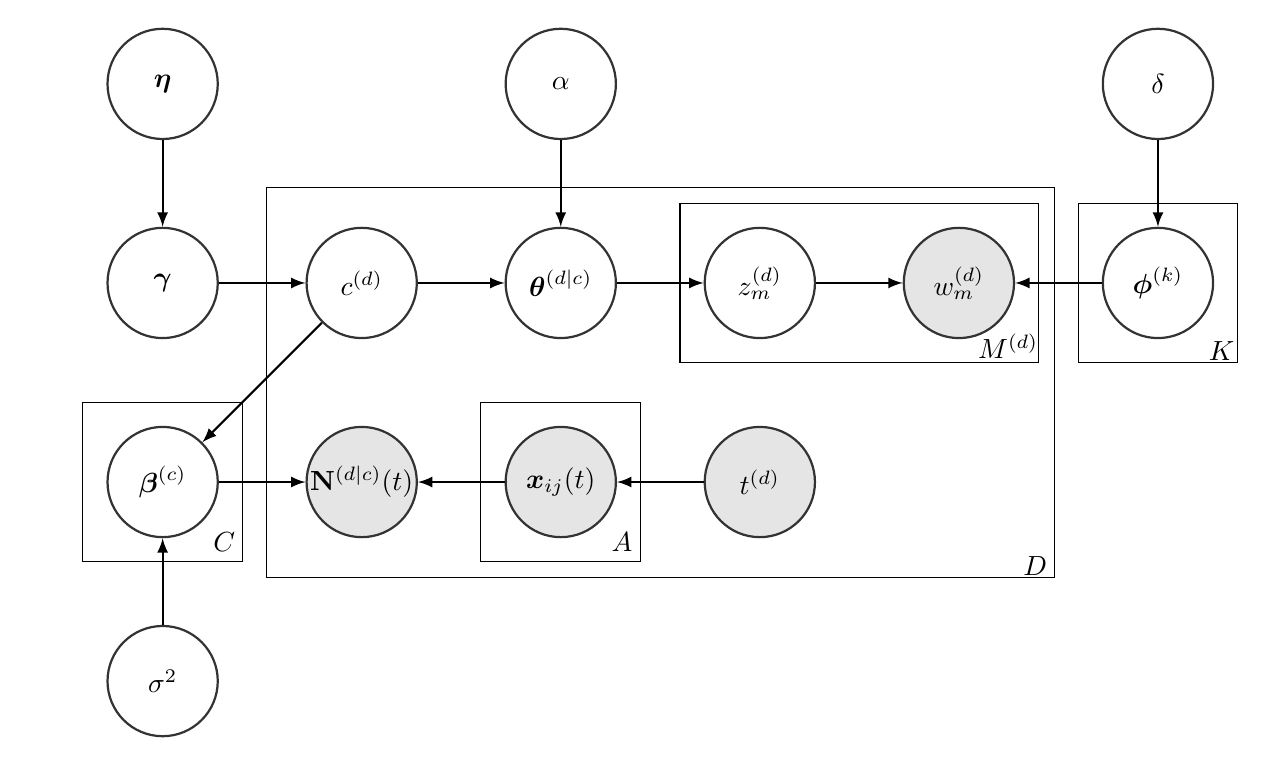
\begin{tikzpicture}
 	\tikzstyle{main}=[circle, minimum size = 14mm, thick, draw =black!80, node distance = 11mm]
 	\tikzstyle{connect}=[-latex, thick]
 	\tikzstyle{box}=[rectangle, draw=black!100]
 	\node[main, fill = white!100] (gamma) [label=center:$\boldsymbol{\gamma}$] { };
 	\node[main] (c) [right=of gamma,label=center:$c^{(d)}$] { };
 		\node[main] (theta) [right=of c,label=center:$\boldsymbol{\theta}^{(d|c)}$] { };
 	\node[main] (z) [right=of theta,label=center:$z_m^{(d)}$] {};
 	\node[main, fill = black!10] (w) [right=of z,label=center:$w_m^{(d)}$] { };
 		 	\node[main] (alpha) [above=of theta,label=center:$\alpha$] { };
 	\node[main] (phi) [right=of w,label=center:$\boldsymbol{\phi}^{(k)}$] { };
 	\node[main] (delta) [above=of phi,label=center:$\delta$] { };
 	 			\node[main] (eta) [above=of gamma,label=center:$\boldsymbol{\eta}$] { };
 	 		 	 			\node[main, fill = black!10] (N) [below=of c ,label=center:$\mathbf{N}^{(d|c)}(t)$] { };
 	 		 	 					\node[main, fill = black!10] (x) [right=of N,label=center:$\boldsymbol{x}_{ij}(t)$] { };
 	 		 	 						\node[main] (beta) [below=of gamma ,label=center:$\boldsymbol{\beta}^{(c)}$] { };
 	 		 	 						 	 		\node[main] (sigma) [below=of beta,label=center:$\sigma^2$] { };
 	 		 	 						\node[main,  fill = black!10] (t) [right=of x,label=center:$t^{(d)}$] { };
 	\path (gamma) edge [connect] (c)
 	(c) edge [connect] (theta)
 	(z) edge [connect] (w)
 	(theta) edge [connect] (z)
 	(alpha) edge [connect] (theta)
 	(phi) edge [connect] (w)
 	(delta) edge [connect] (phi)
 	(sigma) edge [connect] (beta)
 	(x) edge [connect] (N)
 	(beta) edge [connect] (N)
 		(c) edge [connect] (beta)
 		(eta) edge [connect] (gamma)
 		(t) edge [connect] (x);
 			\node[rectangle, inner sep=3mm, fit=  (x),label=below right:$A$, xshift=-5mm, yshift=5mm] {};
 			\node[rectangle, inner sep=3mm,draw=black!100, fit= (beta)] {};
 				\node[rectangle, inner sep=4mm, fit=  (beta) ,label= below right:$C$, xshift=-6mm, yshift=6mm] {};
 	\node[rectangle, inner sep=3mm, draw=black!100, fit= (phi)] {};
 		\node[rectangle, inner sep=3mm, draw=black!100, fit= (x) ] {};
 		\node[rectangle, inner sep=0mm, fit= (phi),label=below right:$K$, xshift=-2mm, yshift=1mm] {};
 	\node[rectangle, inner sep=0mm, fit= (w),label=below right:$M^{(d)}$, xshift=-6mm, yshift=2mm] {};
 	\node[rectangle, inner sep=3mm,draw=black!100, fit= (w)(z)] {};
 	\node[rectangle, inner sep=3mm, fit= (c) (theta) (z) (w) (N) (x) (t),label=below right:$D$, xshift=22mm, yshift=2mm] {};
 	\node[rectangle, inner sep=5mm, draw=black!100, fit = (theta) (c) (z) (w) (N) (x) (t)] {};
 	\end{tikzpicture}
 	\caption{Plate notation of IPTM}
 	\label{fig:plate}
 \end{figure}
 \normalsize
\subsection{Dynamic covariates to measure network effects}
The network statistics $\boldsymbol{x}_t(i, j)$ of equations (2), corresponding to the ordered pair $(i, j)$, can be time-invariant (such as gender) or time-dependent (such as the number of two-paths from $i$ to $j$ just before time $t$). Since time-invariant covariates can be easily specified in various manners (e. g. homophily or group-level effects), here we only consider specification of dynamic covariates.\\ \newline
Following \cite{PerryWolfe2012}, we use 6 effects as components of $\boldsymbol{x}_t(i, j)$. The first two behaviors (send and receive) are dyadic, involving exactly two actors,
while the last four (2-send, 2-receive, sibling, and cosibling) are triadic, involving exactly three actors. However, we take different approach by defining the effects not to be based on finite sub-interval, which require large number of dimention. Instead, we create a single statistic for each effect by incorporating the recency of event into the statistic itself. 
\begin{itemize}[leftmargin=*,rightmargin=-1cm ]
\item [0.] $\mbox{intercept}_t(i, j) = 1$
\item [1.]  $\mbox{send}_t(i, j)=\sum\limits_{d: t^{(d)}<t} I\{i\rightarrow j\}\cdot g(t-t^{(d)})$
\item [2.] $\mbox{receive}_t(i, j)=\sum\limits_{d: t^{(d)}<t} I\{j\rightarrow i\}\cdot g(t-t^{(d)})$
\item [3.] $\mbox{2-send}_t(i, j)=\sum\limits_{h \neq i, j}\Big(\sum\limits_{d: t^{(d)}<t}  I\{i\rightarrow h\}\cdot g(t-t^{(d)})\Big)\Big(\sum\limits_{d: t^{(d)}<t} I\{h\rightarrow j\}\cdot g(t-t^{(d)})\Big)$
\item [4.]  $\mbox{2-receive}_t(i, j)=\sum\limits_{h \neq i, j}\Big(\sum\limits_{d: t^{(d)}<t} I\{h\rightarrow i\}\cdot g(t-t^{(d)})\Big)\Big(\sum\limits_{d: t^{(d)}<t} I\{j\rightarrow h\}\cdot g(t-t^{(d)})\Big)$
\item [5.] $\mbox{sibling}_t(i, j)=\sum\limits_{h \neq i, j}\Big(\sum\limits_{d: t^{(d)}<t} I\{h\rightarrow i\}\cdot g(t-t^{(d)})\Big)\Big(\sum\limits_{d: t^{(d)}<t} I\{h\rightarrow j\}\cdot g(t-t^{(d)})\Big)$
\item [6.] $\mbox{cosibling}_t(i, j)=\sum\limits_{h \neq i, j}\Big(\sum\limits_{d: t^{(d)}<t} I\{i\rightarrow h\}\cdot g(t-t^{(d)})\Big)\Big(\sum\limits_{d: t^{(d)}<t} I\{j\rightarrow h\}\cdot g(t-t^{(d)})\Big)$
\end{itemize}
Here, $g(t-t^{(d)})$ reflects the difference between current time $t$ and the timestamp of previous email $t^{(d)}$, thus measuring the recency. Inspired by the self-exciting Hawkes process, which is often used to model the temporal effect of email data, we can take the exponential kernel $g(t-t^{(d)})=we^{-w(t-t^{(d)})}$ where $w$ is the parameter of speed at
which sender replies to emails, with larger values indicating faster response times. Indeed, $w^{-1}$ is the expected number of hours it takes to reply to a typical email. For simplicity, we can fix $w=1$.
\subsection{Inference}
The inference for IPTM is similar to that of CPME. In this case, what we actually observe are the  tokens $\mathcal{W}=\{\boldsymbol{w}^{(d)} \}_{d=1}^{D}$ and the counting process $\mathcal{N}=\{\boldsymbol{N}^{(d)}(t^{(d)}) \}_{d=1}^{D}.$ Next,  $\mathcal{X}=\{\boldsymbol{x}_{t^{(d)}}(i, j)\}_{d=1}^{D}$ is the metadata, and the latent variables are $\Phi=\{\boldsymbol{\phi}^{(t)}\}_{t=1}^{T}, \Theta=\{\boldsymbol{\theta}^{(d|c)} \}_{d=1}^{D}, \mathcal{Z}=\{\boldsymbol{z}^{(d)} \}_{d=1}^{D}, \mathcal{C}=\{{c}^{(d)} \}_{d=1}^{D},$ and $\mathcal{B}=\{\boldsymbol{\beta}^{(c)} \}_{c=1}^{C}$.\\
\newline 
Below is the the big joint distribution
\begin{equation}
\begin{aligned}
& P(\Phi, \Theta, \mathcal{Z}, \mathcal{W}, \mathcal{C}, \mathcal{B}, \mathcal{N}| \mathcal{X}, \delta, \boldsymbol{n}, \alpha, \boldsymbol{m}, \boldsymbol{\gamma}, \boldsymbol{\eta}, \sigma^2) \\& = P( \mathcal{W}| \mathcal{Z}, \Phi)P(\mathcal{N}|\mathcal{X}, \mathcal{C}, \mathcal{B})P(\mathcal{Z}|\Theta)P(\Phi|\delta, \boldsymbol{n})P(\Theta|\alpha, \boldsymbol{m})P(\mathcal{C}|\boldsymbol{\gamma})P(\boldsymbol{\gamma}|\boldsymbol{\eta})P(\mathcal{B}|\sigma^2)
\end{aligned}
\end{equation}
Now we can integrate out $\Phi$ and $\Theta$ in latent Dirichlet allocation by applying Dirichlet-multinomial conjugacy as we did in CPME. 
\begin{equation}
\propto P( \mathcal{Z}|\delta, \boldsymbol{n}, \alpha, \boldsymbol{m}, \boldsymbol{\gamma}, \boldsymbol{\eta})P(\mathcal{W}|\mathcal{Z})P(\mathcal{N}|\mathcal{X}, \mathcal{C}, \mathcal{B})P(\mathcal{C}|\boldsymbol{\gamma})P(\mathcal{B}|\sigma^2)
\end{equation}
Then, we only have to perform inference over the remaining unobserved latent variables $\mathcal{Z}, \mathcal{C},$ and $\mathcal{B}$, using the equation below:
\begin{equation}
P( \mathcal{Z}, \mathcal{C}, \mathcal{B}|\mathcal{W}, \mathcal{N}, \mathcal{X}, \delta, \boldsymbol{n}, \alpha, \boldsymbol{m}, \boldsymbol{\gamma}, \boldsymbol{\eta}, \sigma^2) \propto P(\mathcal{Z}, \mathcal{C}, \mathcal{B}, \mathcal{W}, \mathcal{N} | \mathcal{X}, \delta, \boldsymbol{n}, \alpha, \boldsymbol{m}, \boldsymbol{\gamma}, \boldsymbol{\eta}, \sigma^2)
\end{equation}
 Gibbs sampling or Metropolis-Hastings algorithm is applied by sequentially resampling each latent variables from their respective conditional posterior.
  \subsubsection{Resampling $\mathcal{C}$}
  The next variable we are going to resample is the document-interaction pattern assignments. The conditional posterior probability we want to calculate is:
  \begin{equation}
  \begin{aligned} & P(c^{(d)}=c|\mathcal{Z}, \mathcal{W}, \mathcal{C}_{\backslash d}, \mathcal{B}, \mathcal{N}, \mathcal{X}, \delta, \boldsymbol{n}, \alpha, \boldsymbol{m}, \boldsymbol{\gamma}, \boldsymbol{\eta}, \sigma^2)\\ &\propto  P(c^{(d)}=c, z^{(d)}_m, w^{(d)}_m, N{(t^{(d)})}|\mathcal{Z}_{\backslash d, m}, \mathcal{W}_{\backslash d, m}, \mathcal{C}_{\backslash d}, \mathcal{B}, \mathcal{N}_{\backslash d}, \mathcal{X}, \delta, \boldsymbol{n}, \alpha, \boldsymbol{m}, \boldsymbol{\gamma}, \boldsymbol{\eta}, \sigma^2)\\ & \propto P(c^{(d)}=c, N{(t^{(d)})}| \mathcal{C}_{\backslash d}, \mathcal{B}, \mathcal{N}_{\backslash d}, \mathcal{X}, \boldsymbol{\gamma}, \boldsymbol{\eta}, \sigma^2) \\ & \propto P(c^{(d)}=c|\boldsymbol{\gamma}, \boldsymbol{\eta}) \times P( N{(t^{(d)})} | \mathcal{C}_{\backslash d}, \mathcal{B}, \mathcal{N}_{\backslash d}, \mathcal{X}, \sigma^2)  \\ & \propto P(c^{(d)}=c|\boldsymbol{\gamma}) \times P( N{(t^{(d)})} | \mathcal{C}_{\backslash d}, \mathcal{B}, \mathcal{N}_{\backslash d}, \mathcal{X}) \\ & =\Big(\prod_{c=1}^{C} \gamma_{c}^{I(c^{(d)}=c)}\Big)\times \mbox{exp}\Big\{{-\big(\sum\limits_{i \in A^{(c^{(d)})}}\sum\limits_{j\in \mathcal{J}^{(c^{(d)})}_{(i, t)}}\lambda_{ij}^{(c^{(d)})}\big)t^{(d)}}\Big\}\cdot \prod_{i \in A^{(c^{(d)})}}\prod_{j\in \mathcal{J}^{(c^{(d)})}_{(i, t)}}\frac{(\lambda_{ij}^{(c^{(d)})}t^{(d)})^{n^{(ij)}}}{n^{(ij)}!} 
 \end{aligned}
  \end{equation}
  	with $\lambda_{ij}^{(c)}=\mbox{exp}\Big\{\boldsymbol{\beta}^{(c)T}\boldsymbol{x}^*_t(i, j)\Big\}\cdot 1\{j \in \mathcal{J}^{(c)}_{(i, t)}\}$. \\\newline
  	Since our $n^{(ij)}$ is either 0 or 1, it can be simplified as below:
  	\begin{equation} \gamma_{c^{(d)}}\times \mbox{exp}\Big\{{-\big(\sum\limits_{i \in A^{(c^{(d)})}}\sum\limits_{j\in \mathcal{J}^{(c^{(d)})}_{(i, t)}}\lambda_{ij}^{(c^{(d)})}\big)t^{(d)}}\Big\}\times \Big(\lambda_{i^{(d)}j^{(d)}}^{(c^{(d)})}t^{(d)}\Big)
  	   \end{equation}
  	  Now, we can speed up the computation time by taking the log of equation (8), which becomes:
  	 
  	    %Of course, we can speed up the computation time by taking the log of equation (12), which is identical to (11).
  	%Here, since we still contain product form in the later part of equaiton (8), we can apply Stirling's approximation for factorials, $\mbox{log}(n!)\approx \mbox{log}(n)-n+1$, and obtain approximate log-conditional probability:
  	%\begin{equation}
  	%\begin{aligned} 
  	%&\approx\mbox{log}\Big\{(\bar{M}^{(k|d)}_{\backslash d, m}+\alpha^{(c^{(d)})}m_k)\cdot \frac{\bar{M}^{(w_m^{(d)}|k)}_{\backslash d, m}+\beta n_v}{\bar{M}^{(k)}_{\backslash d, m}+\beta} \Big\}\\& -t_d\big(\sum\limits_{i \in A^{(c^{(d)})}}\sum\limits_{j\in \mathcal{J}^{(c^{(d)})}_{(i, t)}}\lambda_{ij}^{(c^{(d)})}\big)+\sum_{i \in A^{(c^{(d)})}}\sum_{j\in \mathcal{J}^{(c^{(d)})}_{(i, t)}}\Big(n^{(ij)}\mbox{log}{(\lambda_{ij}^{(c^{(d)})}t_d)}-n^{(ij)}\mbox{log}(n^{(ij)})-n^{(ij)}+1\Big)\\
  	%& = \mbox{log}\Big\{(\bar{M}^{(k|d)}_{\backslash d, m}+\alpha^{(c^{(d)})}m_k)\cdot \frac{\bar{M}^{(w_m^{(d)}|k)}_{\backslash d, m}+\beta n_v}{\bar{M}^{(k)}_{\backslash d, m}+\beta} \Big\}\\& -t_d\big(\sum\limits_{i \in A^{(c^{(d)})}}\sum\limits_{j\in \mathcal{J}^{(c^{(d)})}_{(i, t)}}\lambda_{ij}^{(c^{(d)})}\big)+\sum_{i \in A^{(c^{(d)})}}\sum_{j\in \mathcal{J}^{(c^{(d)})}_{(i, t)}}\Big(n^{(ij)}\big(\mbox{log}(\lambda_{ij}^{(c^{(d)})}t_d)-\mbox{log}(%n^{(ij)})-1\big)+1\Big) 
  	%\end{aligned}
  	%\end{equation}
  	%with $\lambda_{ij}^{(c)}=\lambda_0\cdot %\mbox{exp}(\boldsymbol{\beta}^{(c)T}\boldsymbol{x}_t(i, j))\cdot %1\{j \in \mathcal{J}^{(c)}_{(i, t)}\}$, same as before.
  	
\subsubsection{Resampling $\mathcal{Z}$}
First, the new values of $z^{(d)}_m$ are sampled using the conditional posterior probability of being topic $k$:
\begin{equation}
\begin{aligned} & P(z^{(d)}_m=k|\mathcal{W}, \mathcal{Z}_{\backslash d,m}, \mathcal{C}, \mathcal{B}, \mathcal{N}, \mathcal{X})\\ &\propto P(z^{(d)}_m=k, w^{(d)}_m|\mathcal{W}_{\backslash d, m}, \mathcal{Z}_{\backslash d,m}, \mathcal{C}, \mathcal{B}, \mathcal{N}, \mathcal{X})\\
& \propto P(z^{(d)}_m=k, w^{(d)}_m|\mathcal{W}_{\backslash d, m}, \mathcal{Z}_{\backslash d,m}, C, \delta, \boldsymbol{n}, \alpha, \boldsymbol{m})
\end{aligned}
\end{equation}
where the subscript $``{\backslash d, m}"$ denotes the exclsuion of position $m$ in email $d$. In the last line of equation (9), it is the contribution of LDA, so similar to CPME we can write the conditional probability:
	\begin{equation}
	\begin{aligned} 
	& \propto ({M}^{(k|d)}_{\backslash d, m}+\alpha^{(c^{(d)})}m_k)\cdot \frac{{M}^{(w_m^{(d)}|k)}_{\backslash d, m}+\delta n_v}{{M}^{(k)}_{\backslash d, m}+\delta}
	\end{aligned}
	\end{equation}
\newline 
	For faster computation, we can take the log of the equation (9) and work in log space using the log-conditional probability:
		\begin{equation}
		\begin{aligned} 
		& \mbox{log}({M}^{(k|d)}_{\backslash d, m}+\alpha^{(c^{(d)})}m_k)+\mbox{log}( {{M}^{(w_m^{(d)}|k)}_{\backslash d, m}+\delta n_v)-\mbox{log}({M}^{(k)}_{\backslash d, m}+\delta}) 
		\end{aligned}
		\end{equation}
\subsubsection{Resampling $\mathcal{B}$}
Finally, we wan to update the interaction pattern parameter $\boldsymbol{\beta}^{(c)}$. For this, we will use the Metropolis-Hastings algorithm with a proposal density $Q$ being the multivariate Gaussian distribution, with variance $\sigma^2$, centered on the current values of $\boldsymbol{\beta}^{(c)}$. Then we draw a proposal $\boldsymbol{\beta}'^{(c)}$ at each iteration. Under symmetric proposal distribution (such as multivariate Gaussian), we cancel out Q-ration and obtain the acceptance probability equal to:
\begin{equation}
\begin{split}
& \mbox{Acceptance Probability}=
\begin{cases}  \frac{P(\mathcal{B'}|\mathcal{Z}, \mathcal{W}, \mathcal{C}, \mathcal{N}, \mathcal{X})}{P(\mathcal{B}|\mathcal{Z}, \mathcal{W}, \mathcal{C}, \mathcal{N}, \mathcal{X})}\quad\text{if}  <1\\
1 \quad \text{else}
\end{cases}
\end{split}
\end{equation}
After factorization, we get
\begin{equation}
\begin{aligned}
\frac{P(\mathcal{B'}|\mathcal{Z}, \mathcal{W}, \mathcal{C}, \mathcal{N}, \mathcal{X})}{P(\mathcal{B}|\mathcal{Z}, \mathcal{W}, \mathcal{C}, \mathcal{N}, \mathcal{X})} &=\frac{P(\mathcal{N}|\mathcal{B'}, \mathcal{Z}, \mathcal{W}, \mathcal{C}, \mathcal{X})P(\mathcal{B'})}{P(\mathcal{N}|\mathcal{B}, \mathcal{Z}, \mathcal{W}, \mathcal{C}, \mathcal{X})P(\mathcal{B})}\\&=\frac{P(\mathcal{N}|\mathcal{B'}, \mathcal{C}, \mathcal{X})P(\mathcal{B'})}{P(\mathcal{N}|\mathcal{B}, \mathcal{C}, \mathcal{X})P(\mathcal{B})}.
\end{aligned}
\end{equation}
Since $P(\mathcal{N}|\mathcal{B}, \mathcal{C}, \mathcal{X})$ represents the multivariate counting process contribution in \cite{zocher2006multivariate}, we will use put the equation below: \begin{equation}
\mbox{exp}\Big\{{-\big(\sum\limits_{i \in A^{(c^{(d)})}}\sum\limits_{j\in \mathcal{J}^{(c^{(d)})}_{(i, t)}}\lambda_{ij}^{(c^{(d)})}\big)t_d}\Big\}\cdot \prod_{i \in A^{(c^{(d)})}}\prod_{j\in \mathcal{J}^{(c^{(d)})}_{(i, t)}}\frac{(\lambda_{ij}^{(c^{(d)})}t_d)^{n^{(ij)}}}{n^{(ij)}!}
\end{equation}
we apply later part of the equation (12), which is the probability of observing the edges under the interaction pattern parameters. For $P(\mathcal{B})$, we select a multivarate Gaussian priors as mentioned earlier. The equation we will use for the inference is:
	\begin{equation}
	\begin{aligned} 
	&\mbox{log}(P(\mathcal{B'}))-\mbox{log}(P(\mathcal{B}))\\&-t_d\big(\sum\limits_{i \in A^{(c^{(d)})}}\sum\limits_{j\in \mathcal{J}^{(c^{(d)})}_{(i, t)}}\lambda_{ij}^{(c^{(d)})}\big)+\sum_{i \in A^{(c^{(d)})}}\sum_{j\in \mathcal{J}^{(c^{(d)})}_{(i, t)}}\Big(n^{(ij)}\big(\mbox{log}(\lambda_{ij}^{(c^{(d)})}t_d)-\mbox{log}(n^{(ij)})-1\big)+1\Big), 
	\end{aligned}
	\end{equation}
	and then the log of the acceptance ratio we have is:
		\begin{equation}
		\mbox{log(Acceptance Probability) = min(Log of (13), 0) }
			\end{equation}
To determine whether we accept the proposed update or not, we take the usual approacy, by comparing the log of acceptance ratio we have to the log of a sample from uniform(0,1).
\section{Preliminary Analysis}
Hurricane Sandy was the most destructive hurricane in 2012, which hit North Carolina on late October (October 28, Governor Bev Perdue declared a state of emergency in 24 western counties due to snow and strong winds). In our dataset, there are three counties which cover the date of Hurricane Sandy (October 22, 2012 – November 2, 2012), so we focus on the three counties, since the timestamp of email in this case is much more important than usual case without any disastrous event.
\subsection{Dare County}
\footnotesize
\begin{table}[ht]
	\centering
	\begin{tabular}{ |c|ccc|c| } 
		\hline 
		\textbf{Period} &\textbf{Before Sandy} & \textbf{During Sandy} & \textbf{After Sandy} & \textbf{Overall} \\ 	\hline
			\textbf{\# emails}& 1933 & 1563 & 1467 & 4963 \\ 
		\hline
	\end{tabular}
	\caption{ Summary of Dare county email data based on time period}
	\label{table:nullDare2}
\end{table}
\normalsize
Before Sandy ranges from 2012-09-01 to 2012-10-21 (7 weeks), During Sandy ranges from 2012-10-22 to 2012-11-02 (2 weeks), and After Sandy ranges from 2012-11-03 to 2012-11-30 (4 weeks).
\footnotesize
\begin{figure}[ht]
	\centering
	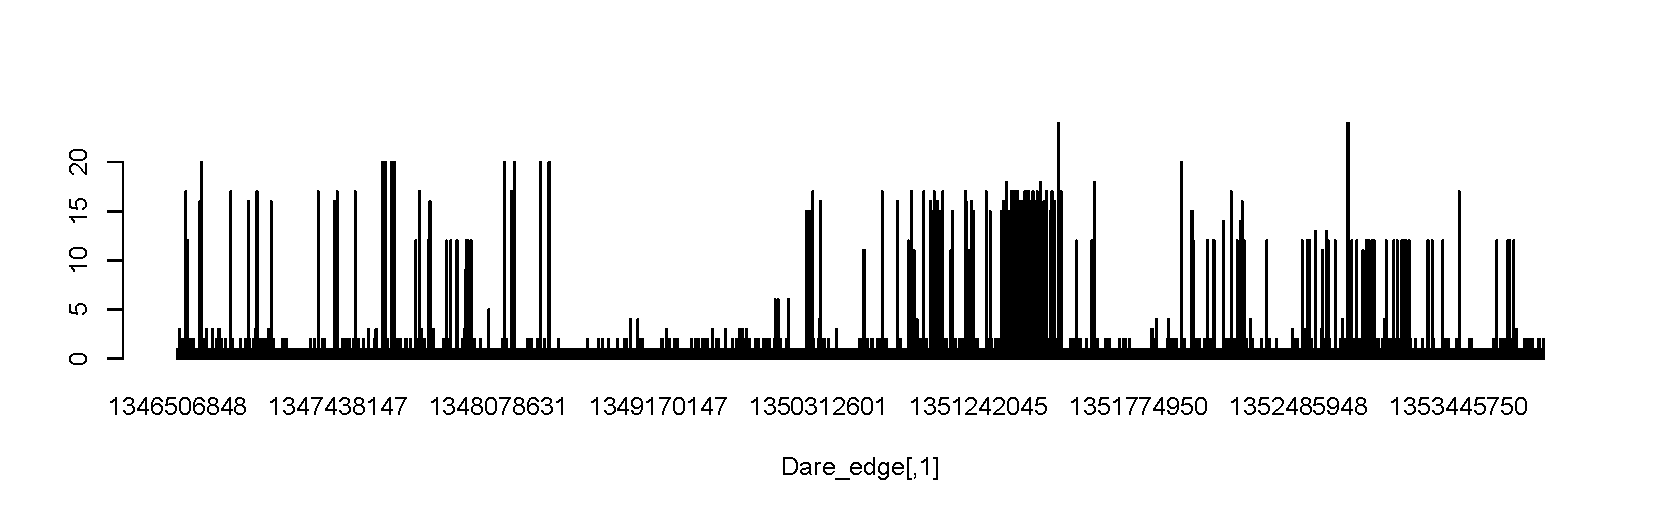
\includegraphics[width=1.1\textwidth]{DareEmails.pdf} 
	\caption{Frequency of Dare county emails from 2012-09-01 to 2012-11-30  }
	\label{fig:Emailplots}
\end{figure}
\begin{table}[ht]
	\centering
	\begin{tabular}{ |c|cc| } 
		\hline 
		\textbf{Time Interval} &\textbf{send} & \textbf{receive} \\ 	
		\hline  $[-\infty, t)$&  2.128, 2.659, 2.355, 2.919& 0.292, 0.257, 0.047, 0.110\\  $[t-30 m, t)$ &  0.262, -0.064, 0.782, 0.317 &2.087, 1.287 , 2.346, 1.870\\  $[t-2h, t-30m)$& 0.383, 0.157 , 0.024, -0.045 &0.553, 0.082, 0.794, 0.269\\ $[t-8h, t-2h)$ & 0.816, 0.054 , 0.077, 0.381 &-0.221, 0.048, 0.298, -0.012 \\ $[t-32h, t-8h)$& 0.085, 0.014,  0.228, 0.070 &0.101, 0.017, -0.033, 0.019\\ $[t-5.33d, t-32h)$&  0.103, 0.025, 0.092, 0.008 &-0.027, -0.016, -0.033, -0.009 \\ $[t-21.33d, t-5.33d)$  & 0.052, 0.000, 0.059, 0.010& 0.013, 0.030 , -0.016, 0.013\\ 
		$[-\infty, t-21.33d)$  & 0.052, 0.103, 0.027, 0.021  & 0.008, 0.000, 0.020, -0.005\\
		\hline
	\end{tabular}
	\caption {Estimated coefficients and approximate standard errors for dyadic effects of Dare county data (before Sandy, during Sandy, after Sandy, overall)}
	\label{table:nullDare}
\end{table}
\footnotesize
\begin{figure}[ht]
	\centering
	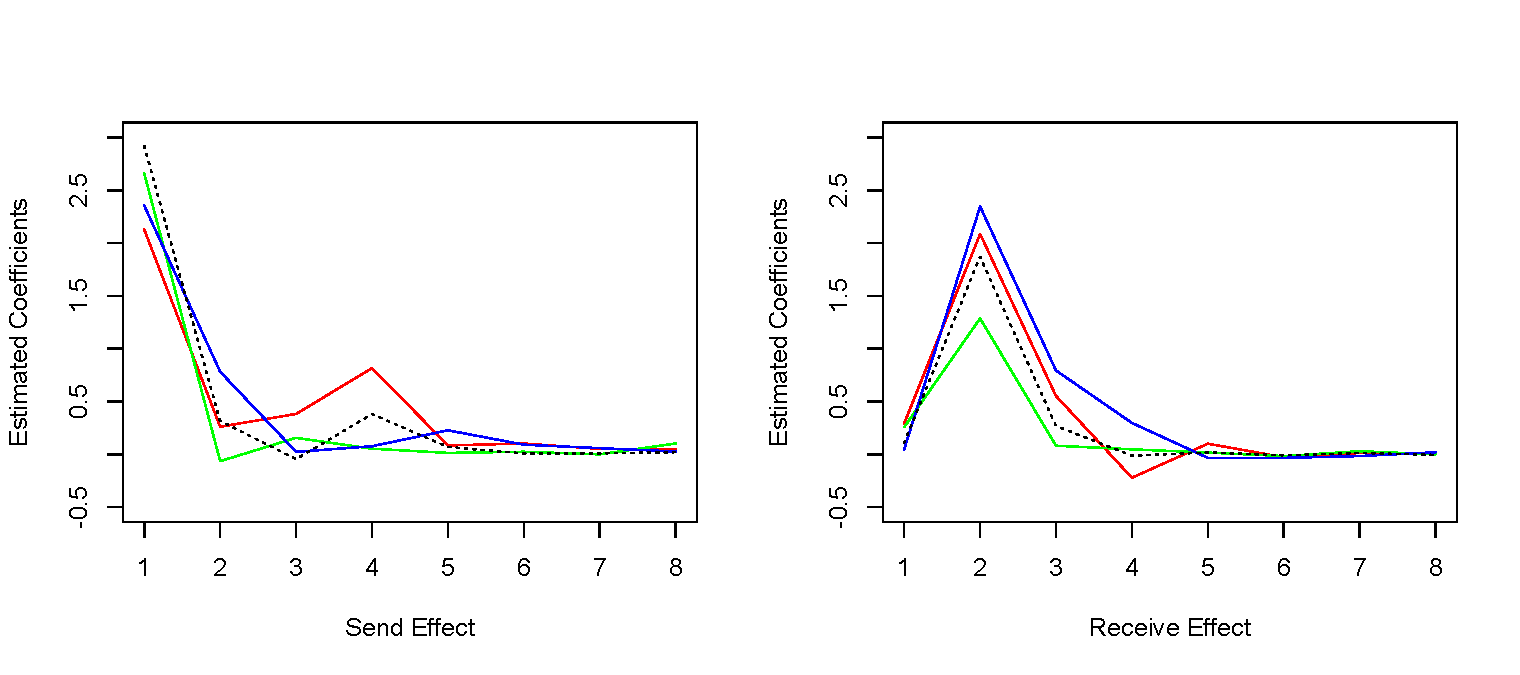
\includegraphics[width=1.1\textwidth]{Dareplot.pdf} 
	\caption{Comparison of Send (left) and Receive (right) effect based on periods in Table 1. (Red=Before, Green=During, Blue=After, and dot=Overall)}	\label{fig:Emailplo22t}
\end{figure}
\subsection{Lenoir County}
\footnotesize
\begin{table}[ht]
	\centering
	\begin{tabular}{ |c|ccc|c| } 
		\hline 
		\textbf{Period} &\textbf{Before Sandy} & \textbf{During Sandy} & \textbf{After Sandy} & \textbf{Overall} \\ 	\hline
		\textbf{\# emails}& 216 & 83 & 302 & 601 \\ 
		\hline
	\end{tabular}
	\caption{ Summary of Lenoir county email data based on time period}
	\label{table:nullDare22}
\end{table}
\normalsize
Before Sandy ranges from 2012-10-01 to 2012-10-21 (3 weeks), During Sandy ranges from 2012-10-22 to 2012-11-02 (2 weeks), and After Sandy ranges from 2012-11-03 to 2012-12-31 (8 weeks).
\footnotesize
\begin{figure}[ht]
	\centering
	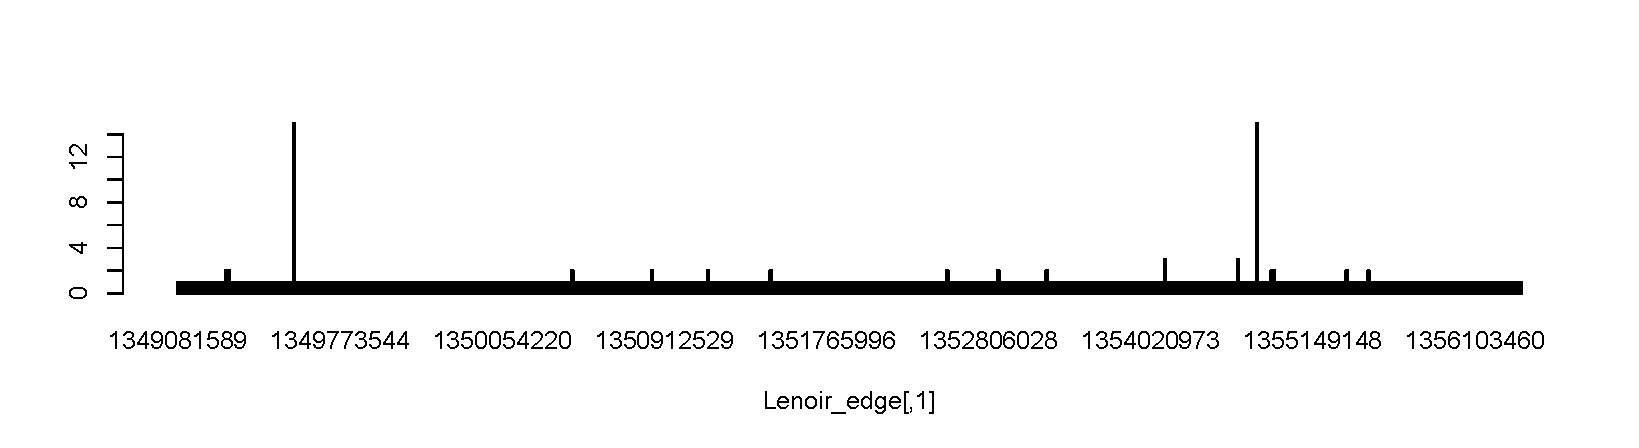
\includegraphics[width=1.1\textwidth]{LenoirEmails.pdf} 
	\caption{Frequency of Lenoir county emails from 2012-10-01 to 2012-12-31  }
	\label{fig:Emailplots32}
\end{figure}
\newpage
\subsection{Vance County}
\footnotesize
\footnotesize
\begin{table}[ht]
	\centering
	\begin{tabular}{ |c|ccc|c| } 
		\hline 
		\textbf{Period} &\textbf{Before Sandy} & \textbf{During Sandy} & \textbf{After Sandy} & \textbf{Overall} \\ 	\hline
		\textbf{\# emails}& 198& 18 & 55 & 271 \\ 
		\hline
	\end{tabular}
	\caption{ Summary of Vance county email data based on time period}
	\label{table:nullVance}
\end{table}
\normalsize
Before Sandy ranges from 2012-09-04 to 2012-10-21 (7 weeks), During Sandy ranges from 2012-10-22 to 2012-11-02 (2 weeks), and After Sandy ranges from 2012-11-03 to 2012-11-30  (4 weeks).
\footnotesize
\begin{figure}[ht]
	\centering
	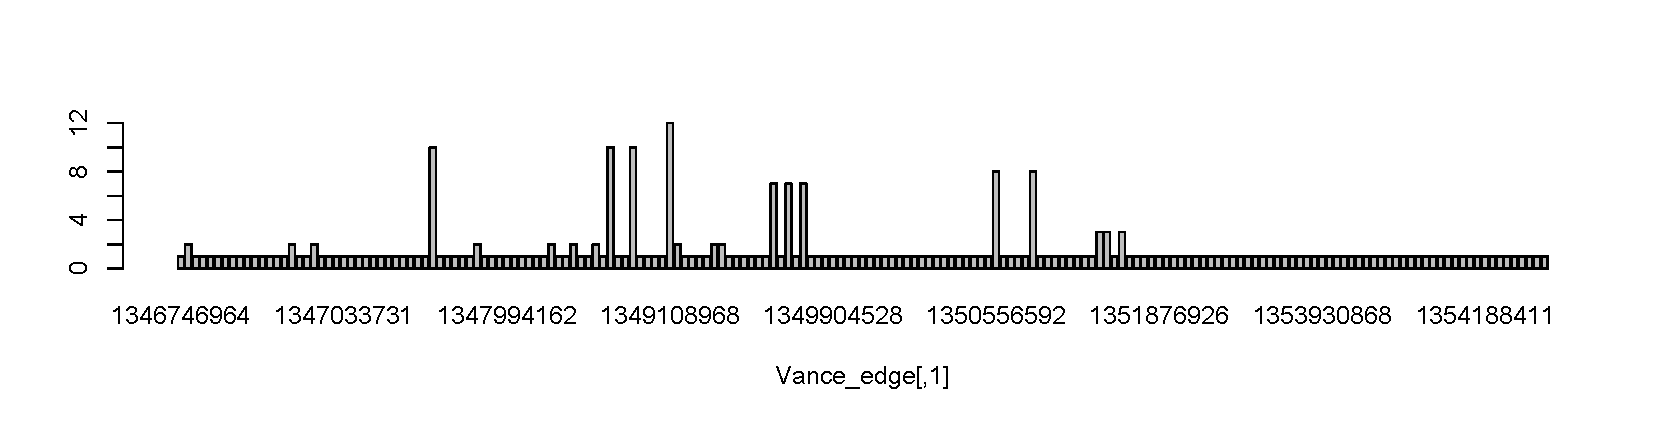
\includegraphics[width=1.1\textwidth]{VanceEmails.pdf} 
	\caption{Frequency of Vance county emails from 2012-09-04 to 2012-11-30  }
	\label{fig:Emailplots22}
\end{figure}
\bibliographystyle{apalike}
\bibliography{BominBib}

\end{document}